\newpage
\section{Initial Event Selection}
\label{sec:InitSelec}
Initial event selection is done to ensure that events that are accepted into the analysis are not contaminated by extremely noisey detector environments and happened during times when the ATLAS detector was accepting events properly.  All of the events  have the same initial set of criteria for determining whether or not the event is looked at any further for this analysis, applying to both MC and Data.  These initial checks are as follows:

\begin{itemize}
\item Only events occuring during runs good for physics
\item Good Calorimeter status: Ensures that the LAr and Tile calorimeters are not experiencing a noise burst at the time of the event
\item Requires a primay vertex to be reconstructed for the event which ensures timing of further reconstructed objects are placed with the correct vertex
\item Global Trigger Decision: Selects events based on wheter they passed one of the triggers including the trigger thresholds, further discussion in Section \ref{sec:GTRIGDEC}
\item Trigger Match: Select events where an electron or muon matches the trigger
\item Overlap Removal as discussed in Section \ref{sec:OverlapRemoval}
\item Ignore events that have a bad muon, occurs mostly in the transition region and the cathode strip chamber regions.
\item Jet Cleaning: Removes events with jets formed from calorimeter information from sources that have nothing to do with the energy flow from the initial hard scatter interaction
\end{itemize}

These basic event selection values are applied to every event, in both MC and Data.  On top of these various kinematic cuts are added to form the additional analysis level objects and regions used in the analysis.  These additional kinematic cuts are examined more closely in Section \ref{sec:preselcuts} and in the discussion of kinematic region creation throughout the rest of the analysis e.g., Section \ref{sec:BkgEvalCRVR}.


\subsection{Triggers}
\label{sec:GTRIGDEC}
Different HLT triggers are used for data taking periods for each year of Run 2.  This analysis takes advantage of single lepton triggers for electrons and muons to dramatically reduce backgrounds due to QCD events without leptons.  

\begin{table}[]
\small
\begin{center}
{\renewcommand{\arraystretch}{1.2}
\begin{tabular}{c|c|c|c|c}
\hline
Year  &  $p_T$ threshold [GeV]   & Identification Menu & Isolation menu & L1 Seed  \\  \hline 
2015   &    $\geq 24  $ &  Medium  &  None	& L1EM20VH	\\
           &   $\geq 60   $ &   Medium  &  None	&  -	\\  
            &  $\geq 120 $ &   Loose  &    None		& -	\\ \hline 
  &   $\geq 26   $ &  Tight  &   Gradient (Loose) 	&  -	\\
2016-2018  &   $\geq 60   $ &   Medium  &  None	&  -	\\  
 &  $\geq 140 $ &   Loose  &  None	&  -	 \\ \hline     
\end{tabular}
\caption{The electron trigger requirements in the event selections}
\label{tab:ElectronTrigs}
}
\end{center}
\end{table}

\begin{table}[]
\small
\begin{center}
{\renewcommand{\arraystretch}{1.2}
\begin{tabular}{c|c|c|c|c}
\hline
Year  &  $p_T$ threshold [GeV]   & Identification Menu & Isolation menu & L1 Seed  \\  \hline 
2015   &    $\geq 20  $ & None  &  Gradient (Loose)	& L1MU15 \\
           &   $\geq 50   $ &   None  &  None	&  -	\\   \hline 
2016-2018  &   $\geq 26   $ &  None  &   Gradient (Medium) 	&  -	\\
  &   $\geq 50   $ &   None  &  None	&  -	\\ \hline   
\end{tabular}
\caption{The muon trigger requirements in the event selections}
\label{tab:MuonTrigs}
}
\end{center}
\end{table}



\subsection{Data and MC Pre-Selection Cuts}
\label{sec:preselcuts}
The Signal Region pre-selection is defined to select events that have an opportunity to enter the final search selection.  This pre-selection selects events with exactly one massive lepton, at least two jets (at least one of which is b-tagged at the 77\% working point), transverse momentum and exactly one photon such that it resembles the expected final-state toplogy for the signal.  All of the events have the same initial set of criteria for determining whether or not the event is looked at any further for this analysis, applying to both MC and Data.  These initial checks are as follows:
%% Preselection Itemization
\begin{itemize}
\item Exactly 1 lepton (electron or muon) $p_T >$ 25 GeV
\item At least two good jets ($p_T >$ 25 GeV)
\item At least one b-tag (MV2c10, 77\% Working point)
\item $\slashed{E}_T >$ 30 GeV and $m_T^W >$ 30 GeV (for events with electrons)
\item $\slashed{E}_T >$ 20 GeV and $\slashed{E}_T + m_T^W >$ 60 GeV (for events with muons)
\item Exactly 1 photon, $p_T >$ 50 GeV %%%%%%%%%%%%%%%%%%%%%%%%%%%%%%%%%% Change if change plots
\end{itemize}

These plots are also produced before additional scale factors to account for mismodelling of various processes are taken into account.  These include the fake rate scale factors for processes where a truth electron or hadron are reconstructed to a photon and scaling to account for further mismodeling based on the order of the MC events produced (leading order, next-to-leading order, etc.).  Only statistical uncertainties are shown

Signal photons, which originate from a top quark decay, are very high $p_T$ whereas background photons typically result from soft processes.  A cut on the photon candidate $p_T$ removes much of the backgrounds while keeping a majority of the signal.  The photon $p_T$ in the preselection region is shown in Figure \ref{fig:PreSelPlots1}.  
%%SR Pre Selection Plots
\begin{figure}[h!]
\centering
\subfloat[electron channel]{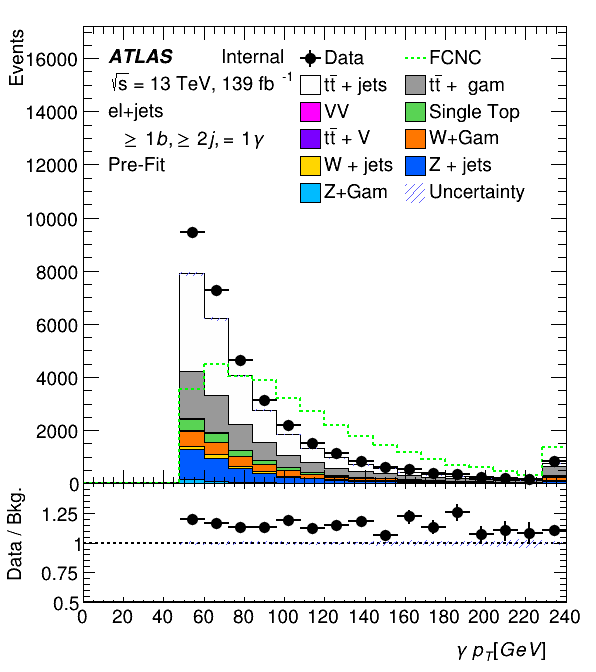
\includegraphics[width=.45\columnwidth]{../ThesisImages/RegionPlots/BeforeScaling/PreSelection/FCNC_All_ejets/Plots/PreSel_ph_pt.png}}\hfil
\subfloat[muon channel]{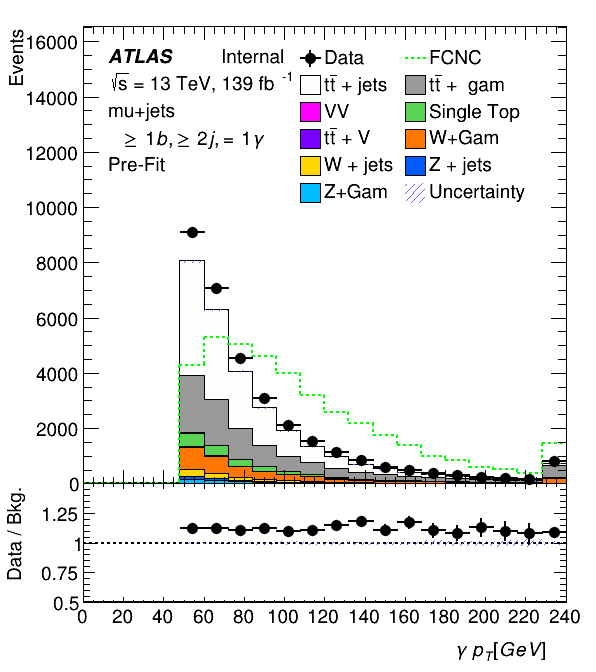
\includegraphics[width=.45\columnwidth]{../ThesisImages/RegionPlots/BeforeScaling/PreSelection/FCNC_All_mujets/Plots/PreSel_ph_pt.png}}
\caption{Photon $p_T$ in the signal region pre-preselection region.  FCNC signal branching ratio is scaled to 1\%.}
\label{fig:PreSelPlots1}
\end{figure}

Other variables of interest, i.e. those being used as inputs into the neural network are also showed in this section.  Figure \ref{fig:PreSelPlotsST} shows the $S_T$ and $m_T^W$ distributions.  Figure \ref{fig:PreSelTopMasses} shows the invariant mass distributions for both top quark candidates, $m_{Wb}$ and $m_{q\gamma}$.  The kinematic variables for the electron channel are shown in Figure \ref{fig:PreSelPlots2} and for the muon channel in Figure \ref{fig:PreSelPlots3}.  The neural network output of these events are shown in Figure \ref{fig:PreSelPlots5}

\begin{figure}[h!]
\centering
\subfloat[electron channel]{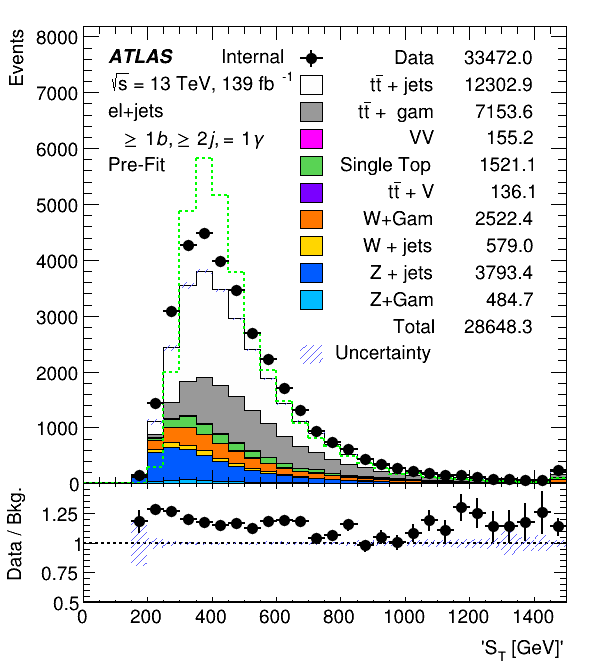
\includegraphics[width=.5\columnwidth]{../ThesisImages/RegionPlots/BeforeScaling/PreSelection/FCNC_All_ejets/Plots/PreSel_ST.png}}\hfil
\subfloat[muon channel]{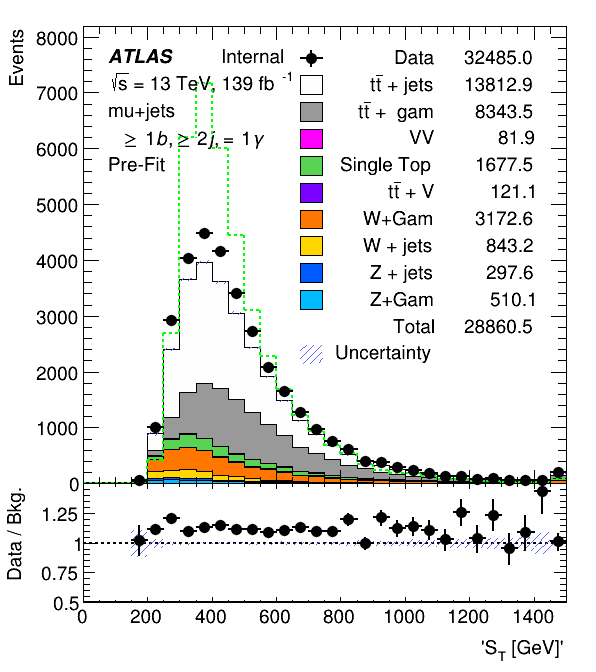
\includegraphics[width=.5\columnwidth]{../ThesisImages/RegionPlots/BeforeScaling/PreSelection/FCNC_All_mujets/Plots/PreSel_ST.png}}
\vspace{-3.mm} \setcounter{subfigure}{0}
\subfloat[electron channel]{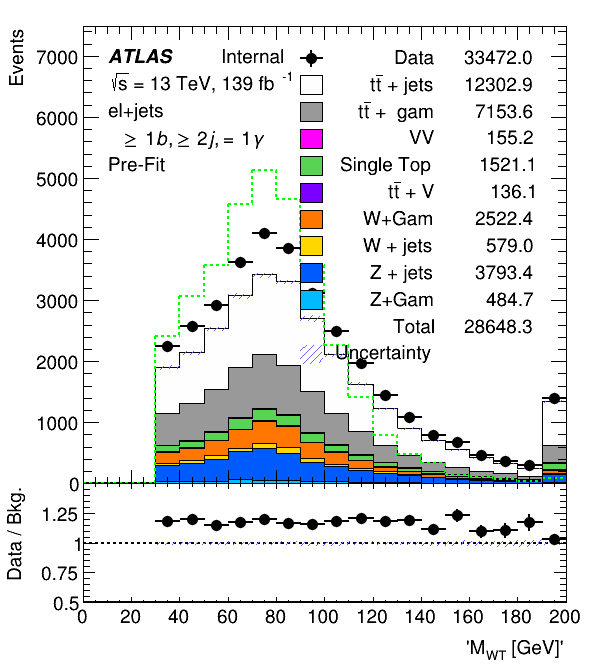
\includegraphics[width=.45\columnwidth]{../ThesisImages/RegionPlots/BeforeScaling/PreSelection/FCNC_All_ejets/Plots/PreSel_MWT.png}}\hfil
\subfloat[muon channel]{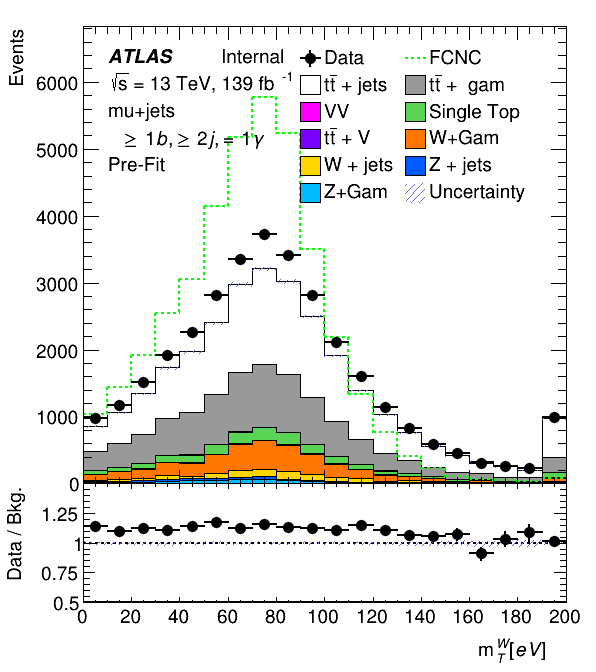
\includegraphics[width=.45\columnwidth]{../ThesisImages/RegionPlots/BeforeScaling/PreSelection/FCNC_All_mujets/Plots/PreSel_MWT.png}}
\caption{$S_T$ and $m_T^W$ in the signal region pre-selection region.  FCNC signal branching ratio is scaled to 1\%.}
\label{fig:PreSelPlotsST}
\end{figure}

\begin{figure}[h!]
\centering
\subfloat{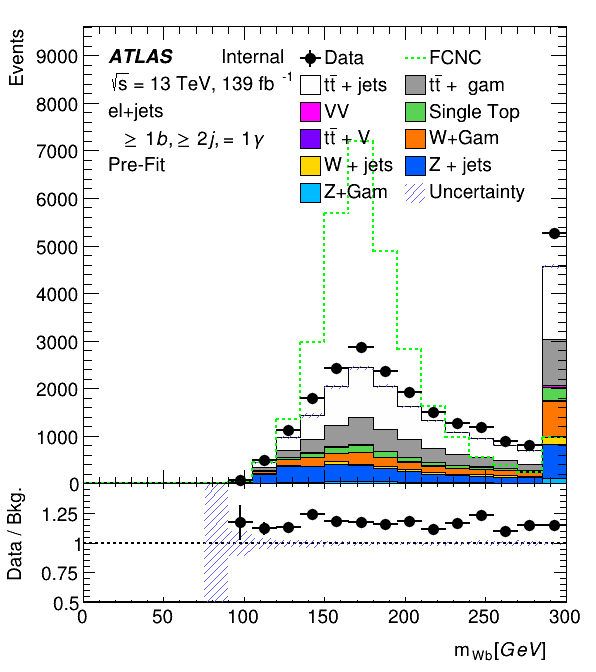
\includegraphics[width=.5\columnwidth]{../ThesisImages/RegionPlots/BeforeScaling/PreSelection/FCNC_All_ejets/Plots/PreSel_SMtop.png}}\hfil
\subfloat{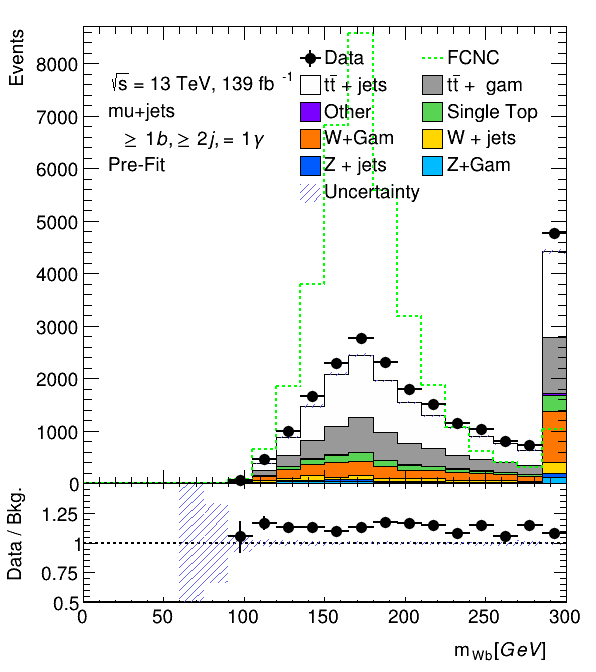
\includegraphics[width=.5\columnwidth]{../ThesisImages/RegionPlots/BeforeScaling/PreSelection/FCNC_All_mujets/Plots/PreSel_SMtop.png}}
\vspace{-3.mm} \setcounter{subfigure}{0}
\subfloat[electron channel]{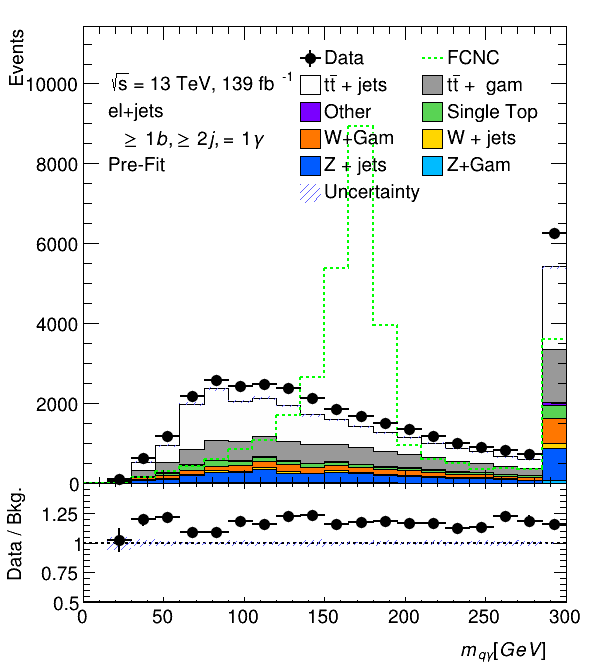
\includegraphics[width=.5\columnwidth]{../ThesisImages/RegionPlots/BeforeScaling/PreSelection/FCNC_All_ejets/Plots/PreSel_mqph.png}}\hfil
\subfloat[muon channel]{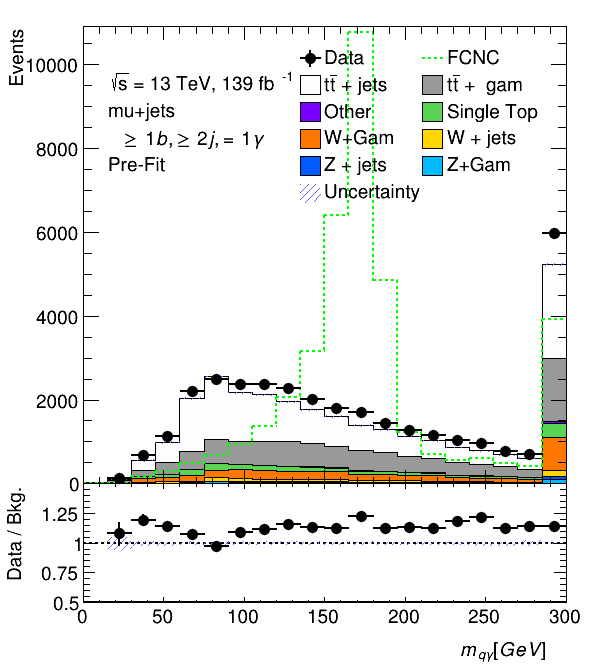
\includegraphics[width=.5\columnwidth]{../ThesisImages/RegionPlots/BeforeScaling/PreSelection/FCNC_All_mujets/Plots/PreSel_mqph.png}}
\caption{Top mass candidates in the signal region pre-selection: $m_{W b}$ and $m_{q\gamma}$. FCNC signal branching ratio is scaled to 1\%.}
\label{fig:PreSelTopMasses}
\end{figure}


%\begin{figure}[h!]
%\centering
%\subfloat{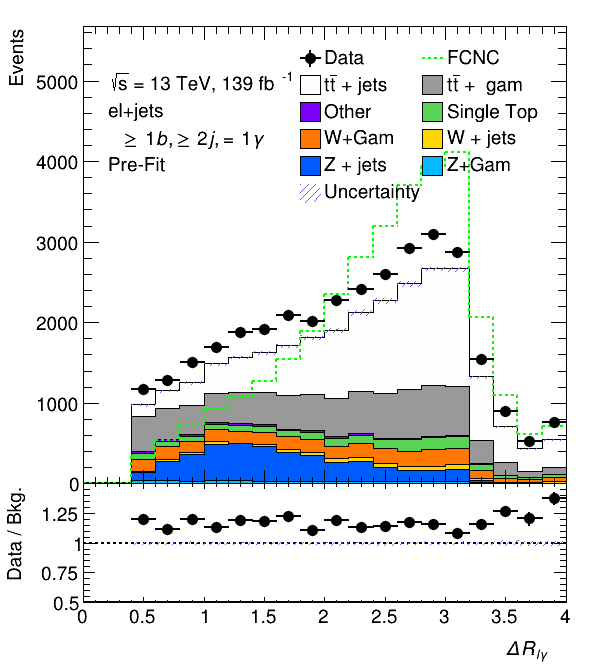
\includegraphics[width=.5\columnwidth]{../ThesisImages/RegionPlots/BeforeScaling/PreSelection/FCNC_All_ejets/Plots/PreSel_drlph.png}}\hfil
%\subfloat{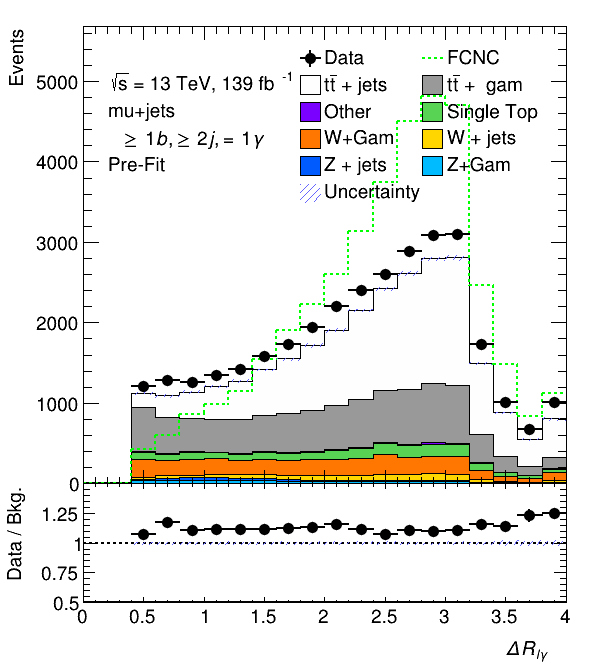
\includegraphics[width=.5\columnwidth]{../ThesisImages/RegionPlots/BeforeScaling/PreSelection/FCNC_All_mujets/Plots/PreSel_drlph.png}}
%\vspace{-3.mm} \setcounter{subfigure}{0}
%\subfloat[electron channel]{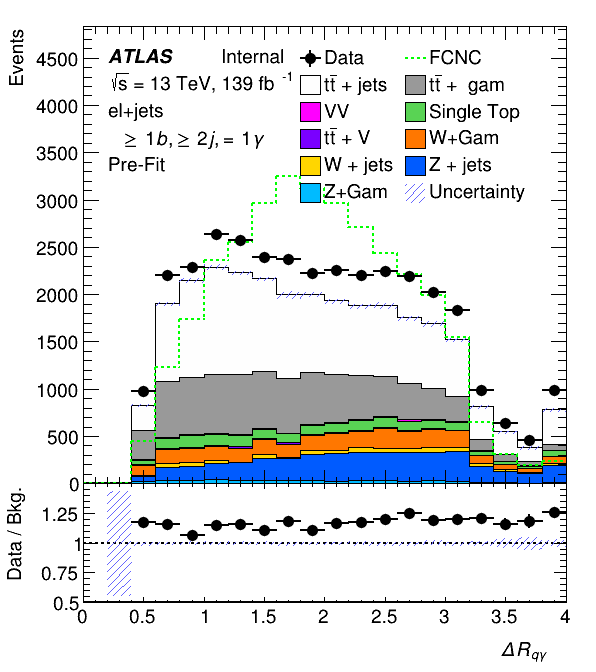
\includegraphics[width=.5\columnwidth]{../ThesisImages/RegionPlots/BeforeScaling/PreSelection/FCNC_All_ejets/Plots/PreSel_drqph.png}}\hfil
%\subfloat[muon channel]{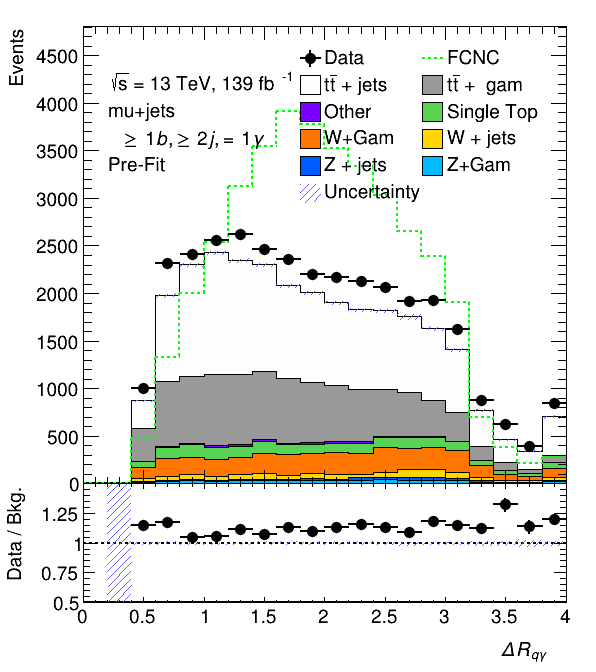
\includegraphics[width=.5\columnwidth]{../ThesisImages/RegionPlots/BeforeScaling/PreSelection/FCNC_All_mujets/Plots/PreSel_drqph.png}}
%\caption{Distance between the photon and closest light jet, $\Delta R_{l \gamma}$, and closest light jet, $\Delta R_{q\gamma}$, in the signal region pre-selection region.  FCNC signal branching ratio is scaled to 1\%}
%\label{fig:PreSeDeltaRs}
%\end{figure}


\begin{figure}[h!]
\centering
\subfloat[]{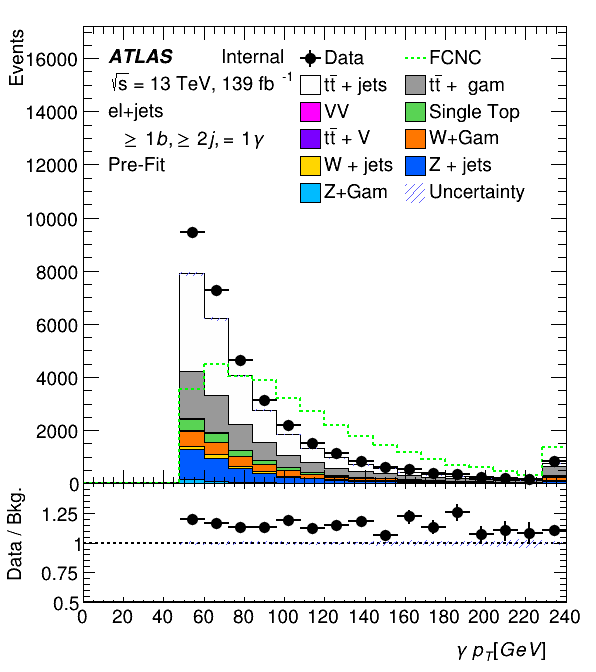
\includegraphics[width=.33\columnwidth]{../ThesisImages/RegionPlots/BeforeScaling/PreSelection/FCNC_All_ejets/Plots/PreSel_ph_pt.png}} \hfil
\subfloat[]{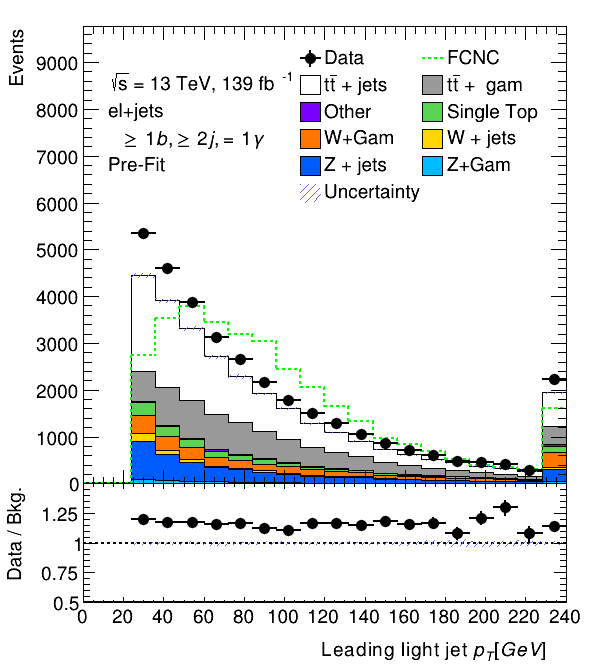
\includegraphics[width=.33\columnwidth]{../ThesisImages/RegionPlots/BeforeScaling/PreSelection/FCNC_All_ejets/Plots/PreSel_jet0_pt.png}} \hfil  
\subfloat[]{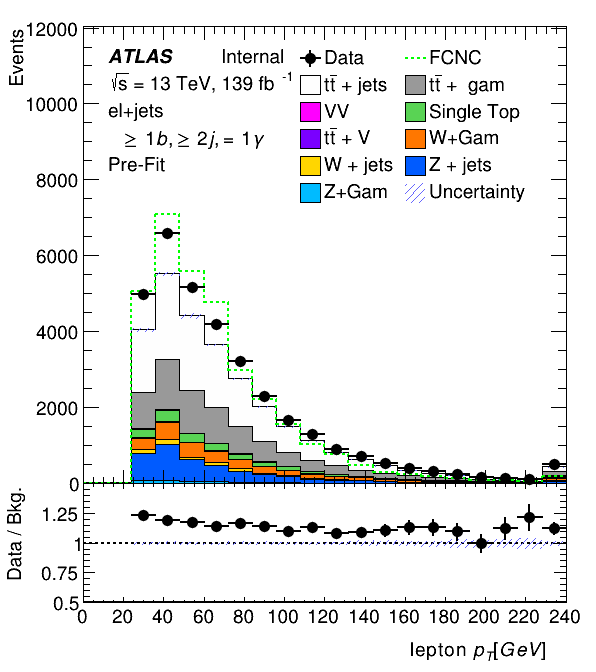
\includegraphics[width=.33\columnwidth]{../ThesisImages/RegionPlots/BeforeScaling/PreSelection/FCNC_All_ejets/Plots/PreSel_lep_pt.png}}
\vspace{-3.mm}
\subfloat[]{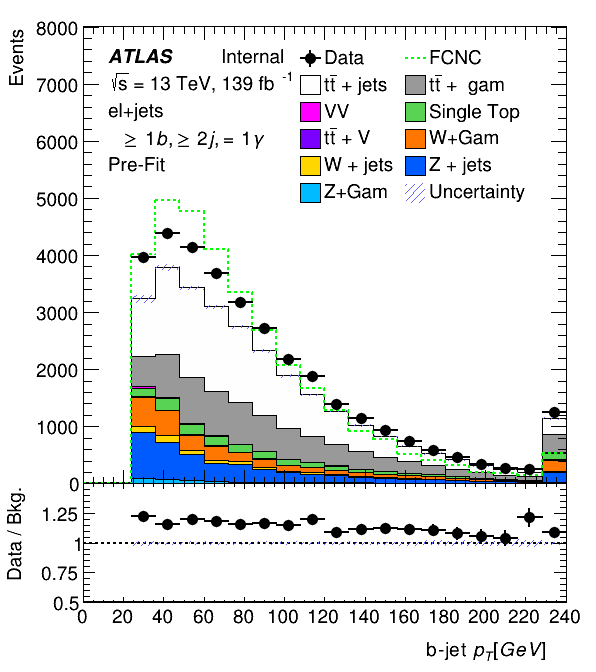
\includegraphics[width=.33\columnwidth]{../ThesisImages/RegionPlots/BeforeScaling/PreSelection/FCNC_All_ejets/Plots/PreSel_bjet0_pt.png}}\hfil
\subfloat[]{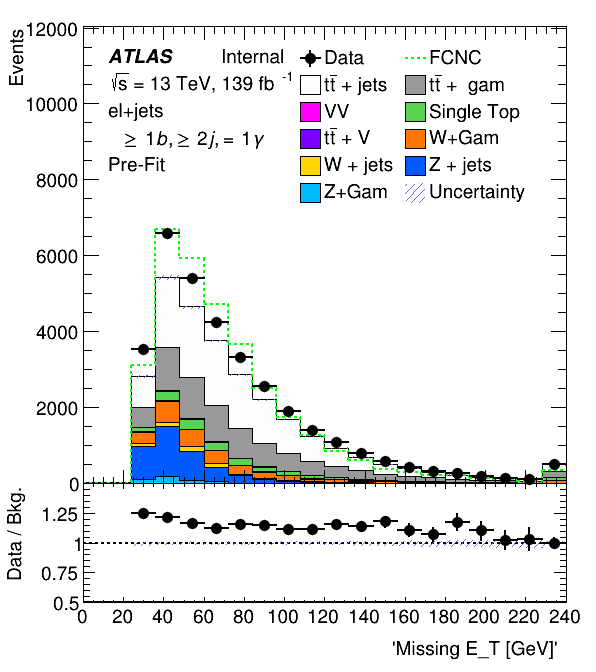
\includegraphics[width=.33\columnwidth]{../ThesisImages/RegionPlots/BeforeScaling/PreSelection/FCNC_All_ejets/Plots/PreSel_met.png}}\hfil
\subfloat[]{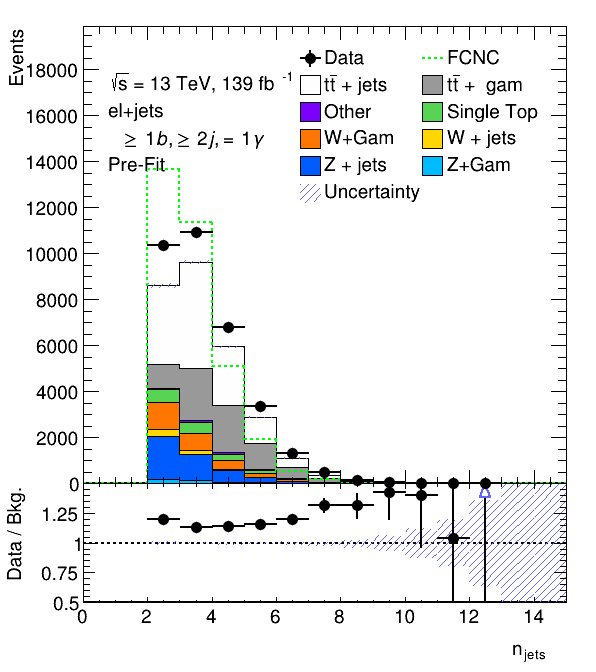
\includegraphics[width=.33\columnwidth]{../ThesisImages/RegionPlots/BeforeScaling/PreSelection/FCNC_All_ejets/Plots/PreSel_njet.png}}
\caption{Photon $p_T$ (a), leading light jet $p_T$ (b), lepton $p_T$ (c), b-jet $p_T$(d), $\slashed{E}_T$ (e), and $n_{\text{jets}}$ (f) plots in the signal region pre-selection for the electron+jets channel.  FCNC signal branching ratio is scaled to 1\%. }
\label{fig:PreSelPlots2}
\end{figure}


\begin{figure}[h!]
\centering
\subfloat[]{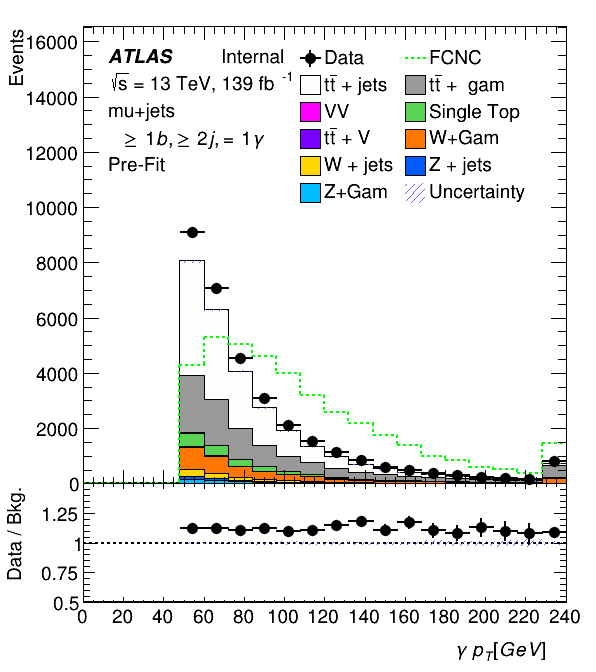
\includegraphics[width=.33\columnwidth]{../ThesisImages/RegionPlots/BeforeScaling/PreSelection/FCNC_All_mujets/Plots/PreSel_ph_pt.png}}\hfil
\subfloat[]{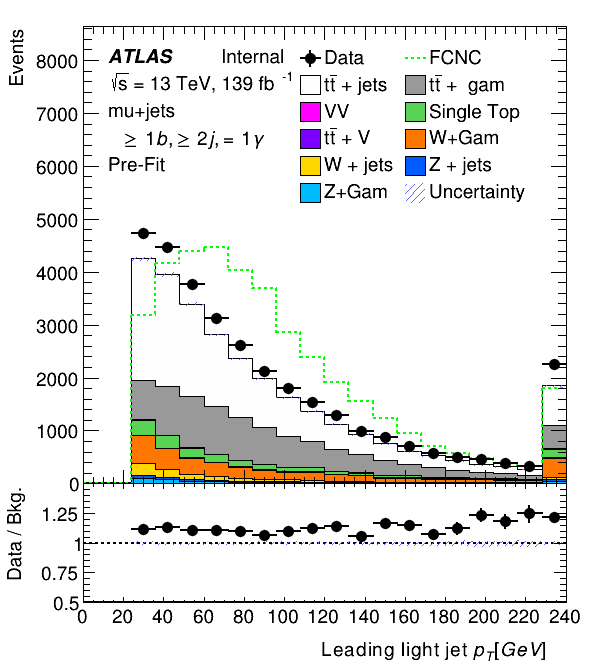
\includegraphics[width=.33\columnwidth]{../ThesisImages/RegionPlots/BeforeScaling/PreSelection/FCNC_All_mujets/Plots/PreSel_jet0_pt.png}}\hfil  
\subfloat[]{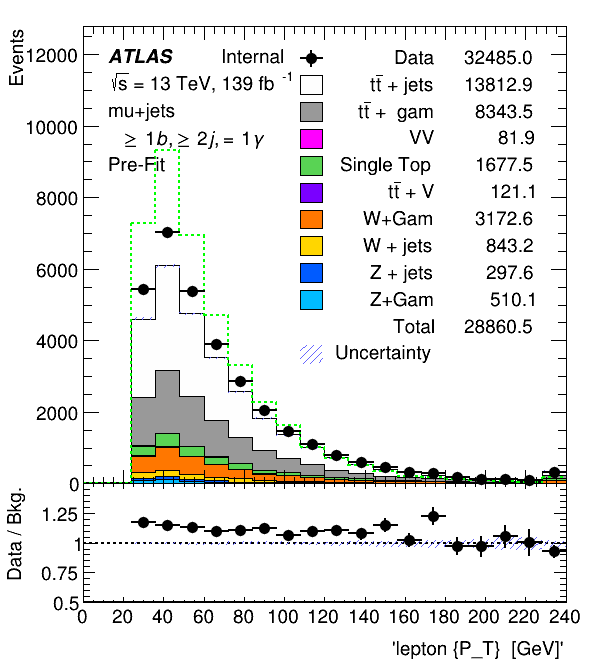
\includegraphics[width=.33\columnwidth]{../ThesisImages/RegionPlots/BeforeScaling/PreSelection/FCNC_All_mujets/Plots/PreSel_lep_pt.png}}
\vspace{-3.mm}
\subfloat[]{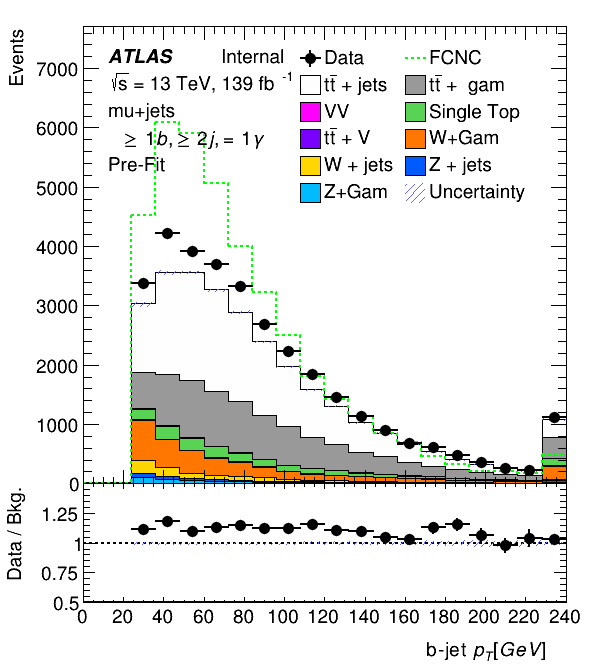
\includegraphics[width=.33\columnwidth]{../ThesisImages/RegionPlots/BeforeScaling/PreSelection/FCNC_All_mujets/Plots/PreSel_bjet0_pt.png}}\hfil
\subfloat[]{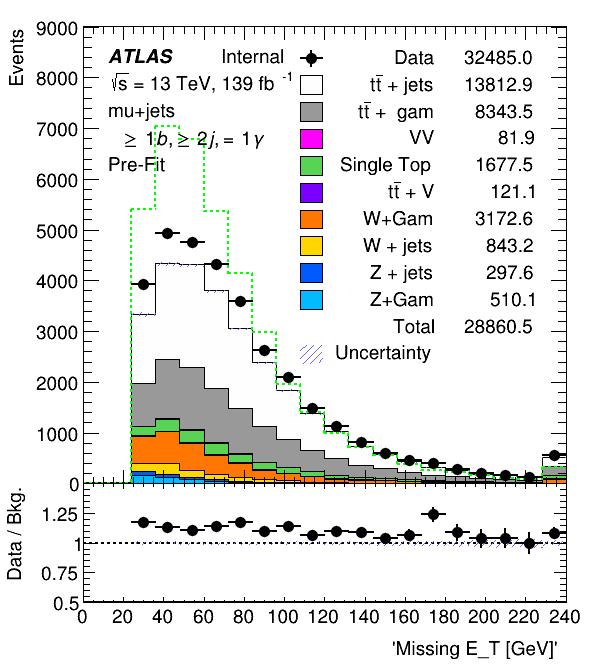
\includegraphics[width=.33\columnwidth]{../ThesisImages/RegionPlots/BeforeScaling/PreSelection/FCNC_All_mujets/Plots/PreSel_met.png}}\hfil
\subfloat[]{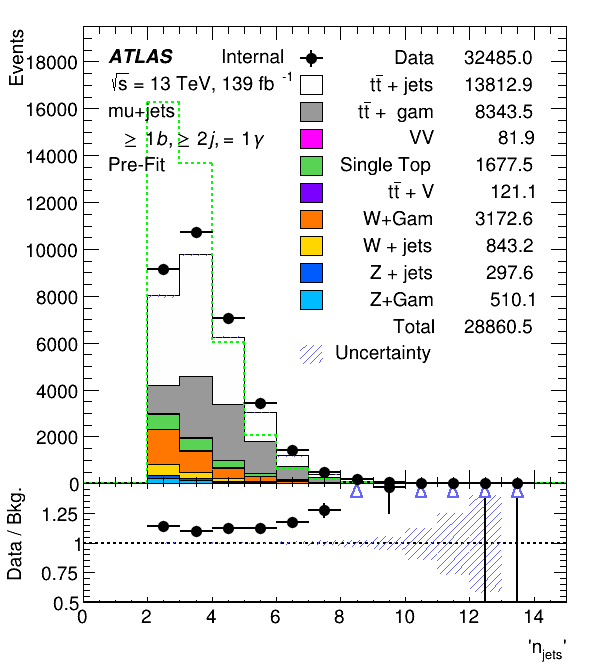
\includegraphics[width=.33\columnwidth]{../ThesisImages/RegionPlots/BeforeScaling/PreSelection/FCNC_All_mujets/Plots/PreSel_njet.png}}
\caption{Photon $p_T$ (a), leading light jet $p_T$ (b), lepton $p_T$ (c), b-jet $p_T$(d), $\slashed{E}_T$ (e), and $n_{\text{jets}}$ (f) plots in the signal region pre-selection for the muon+jets channel.  FCNC signal branching ratio is scaled to 1\%.}
\label{fig:PreSelPlots3}
\end{figure}

\begin{figure}[h!]
\centering
\subfloat[electron channel]{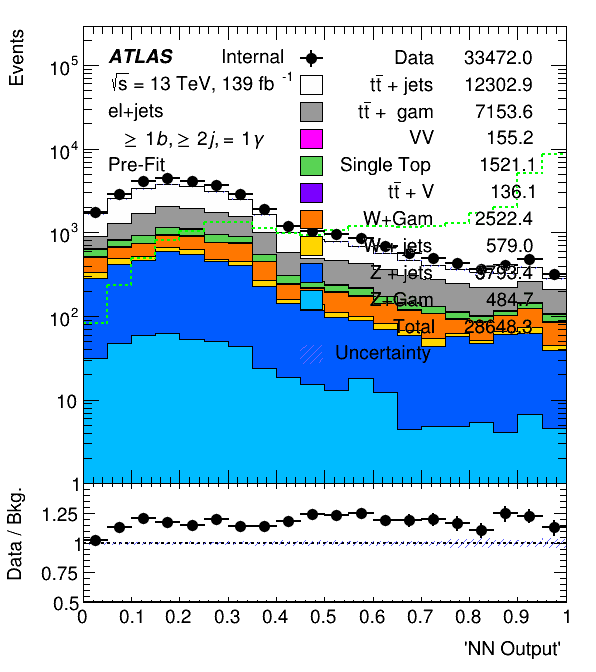
\includegraphics[width=.5\columnwidth]{../ThesisImages/RegionPlots/BeforeScaling/PreSelection/FCNC_All_ejets/Plots/PreSel_NNejet.png}}\hfil
\subfloat[muon channel]{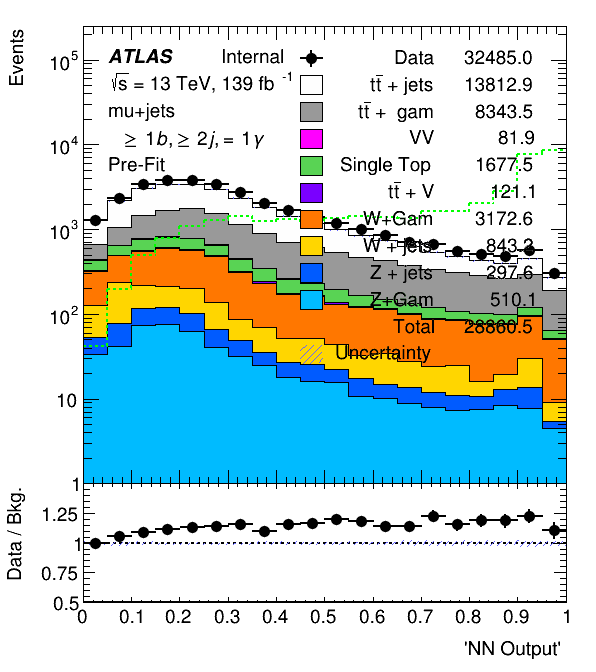
\includegraphics[width=.5\columnwidth]{../ThesisImages/RegionPlots/BeforeScaling/PreSelection/FCNC_All_mujets/Plots/PreSel_NNmujet.png}}
\caption{Output of the Neural Network in the signal region pre-selection region.  FCNC signal branching ratio is scaled to 1\%.}
\label{fig:PreSelPlots5}
\end{figure}

\subsection{Background Evaluation: Control and Validation Regions}
\label{sec:BkgEvalCRVR}
Orthogonal regions to the signal region have been created to test the preformance of Monte Carlo samples.  Control and validation regions are designed to isolate specific physics processes to determine and test the efficacy of scale factors that will be applied to the final signal region Monte Carlo evets.  These control and validation regions need to be kinematically similar to the signal region such that derived scale factors can be translated directly into the signal region and orthogonal to make sure that there is little signal contamination in the regions.  Regions have been made to test the major backgrounds expected in the signal region: $t\bar{t}$, W+jets, as well as events similar events produced with an associated photon: $t\bar{t}+\gamma$ and W+Jets+$\gamma$.  Events without real photons are described in Section \ref{sec:BKGnoPho} and regions with a real photon are described in Section \ref{sec:BKGPho}.

\subsubsection{Backgrounds Without Photons}
\label{sec:BKGnoPho}
Various background processes that do not have a real photon produced in the events can still enter the signal region if an electron or jet is mis-reconstructed as a photon.  Of these processes the largest contributors in the signal region are Standard Model $t\bar{t}$ and W+jets.  As the LHC attains higher and higher energies the QCD multijet backgrounds become increasingly hard to model due to the non-perturbative nature of the interactions.  A data-driven technique for accounting for these backgrounds is developed by scaling the major backgrounds to account for the QCD backgrounds that contribute extra jets to the major backgrounds.  Designing a single control region satisfactorily close to the signal region is impossible.  Thus, two control regions are designed, one which is W+jets rich and the other $t\bar{t}$ rich.  Scale factors for these backgrounds are derived simultaneously and tested in a third similar region for validation before being applied to other regions.  
These control and validation regions are defined as follows:
\begin{itemize}
\item All of the Initial Event Selection as outlined in Section \ref{sec:InitSelec}
\item Exactly 1 lepton (electron or muon) $p_T >$ 25 GeV
\item Number of Jets  ($p_T >$ 25 GeV) to define the regions
	\begin{itemize}
	\item Control Region 1 (W+Jets enriched): $n_{\text{jets}} = 3$
	\item Validation Region: $n_{\text{jets}} =4$
	\item Control Region 2 ($t\bar{t}$ enriched): $n_{\text{jets}} \geq 5$
	\end{itemize}
\item $\slashed{E}_T >$ 30 GeV and $m_T^W >$ 30 GeV (for events with electrons)
\item $\slashed{E}_T >$ 20 GeV and $\slashed{E}_T + m_T^W >$ 60 GeV (for events with muons)
\item Exactly 1 b-tagged jet (MV2c10, 77\% Working point)
\item 0 photons, $p_T >$ 15 GeV
\end{itemize}

\begin{figure}[h!]
\centering
\subfloat[]{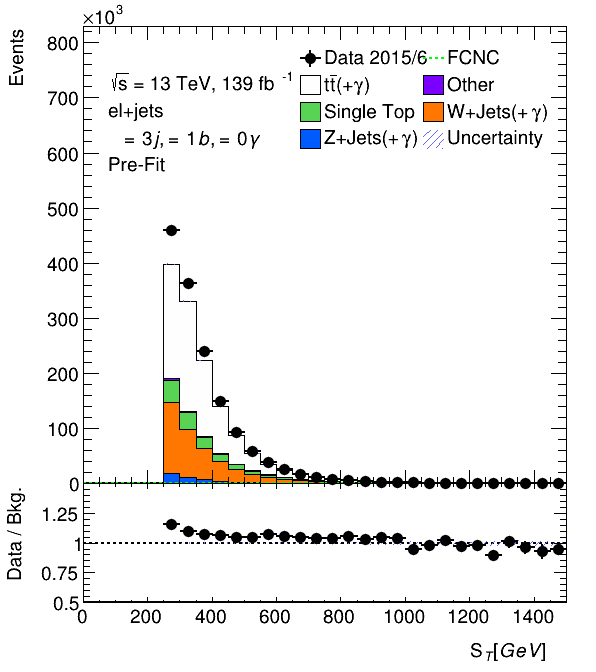
\includegraphics[width=.33\columnwidth]{../ThesisImages/RegionPlots/AfterScaling/ControlRegions/HardCodedNormFactor/FCNC_All_ejets/Plots/CR1_ST.png}}\hfil
\subfloat[]{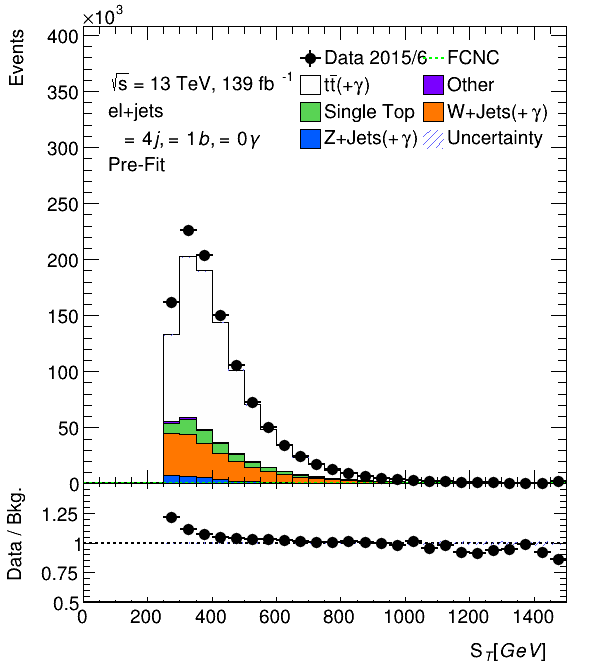
\includegraphics[width=.33\columnwidth]{../ThesisImages/RegionPlots/AfterScaling/ControlRegions/HardCodedNormFactor/FCNC_All_ejets/Plots/VR3_ST.png}}\hfil  
\subfloat[]{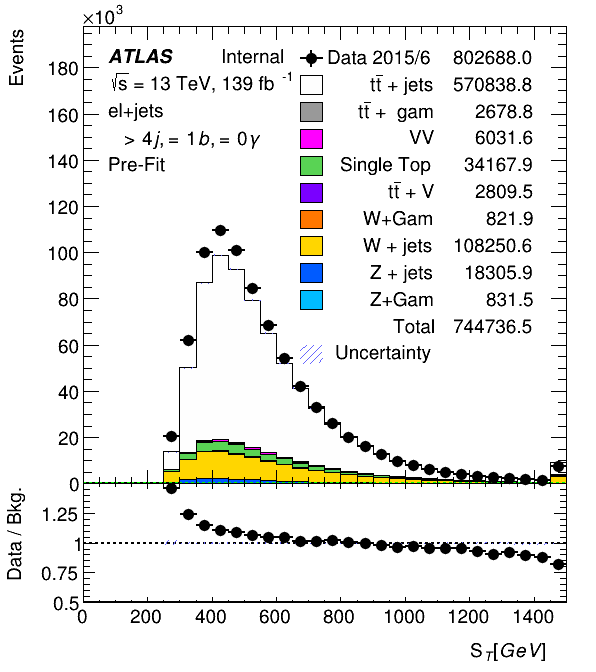
\includegraphics[width=.33\columnwidth]{../ThesisImages/RegionPlots/AfterScaling/ControlRegions/HardCodedNormFactor/FCNC_All_ejets/Plots/CR2_ST.png}}
\vspace{-3.mm}
\subfloat[]{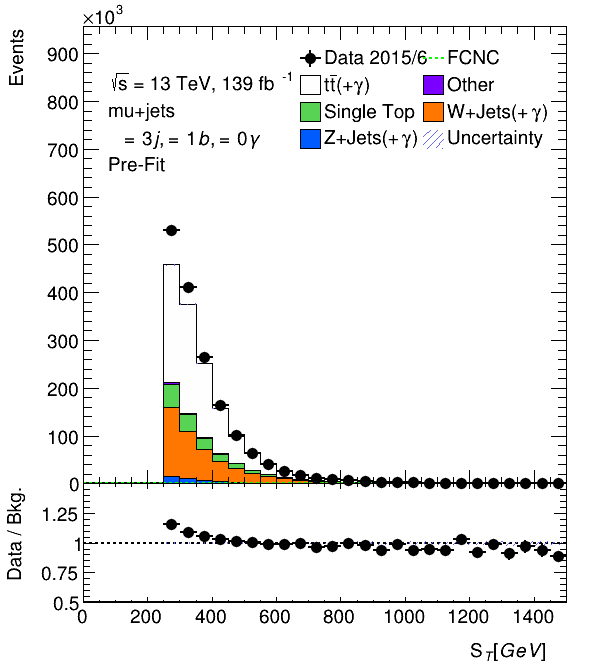
\includegraphics[width=.33\columnwidth]{../ThesisImages/RegionPlots/AfterScaling/ControlRegions/HardCodedNormFactor/FCNC_All_mujets/Plots/CR1_ST.png}}\hfil
\subfloat[]{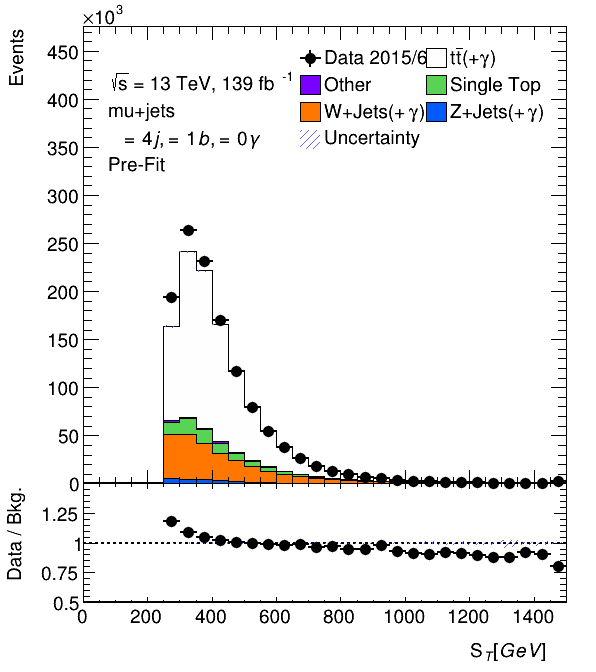
\includegraphics[width=.33\columnwidth]{../ThesisImages/RegionPlots/AfterScaling/ControlRegions/HardCodedNormFactor/FCNC_All_mujets/Plots/VR3_ST.png}}\hfil   %Change from ST Distributions to something at looks more reasonable?
\subfloat[]{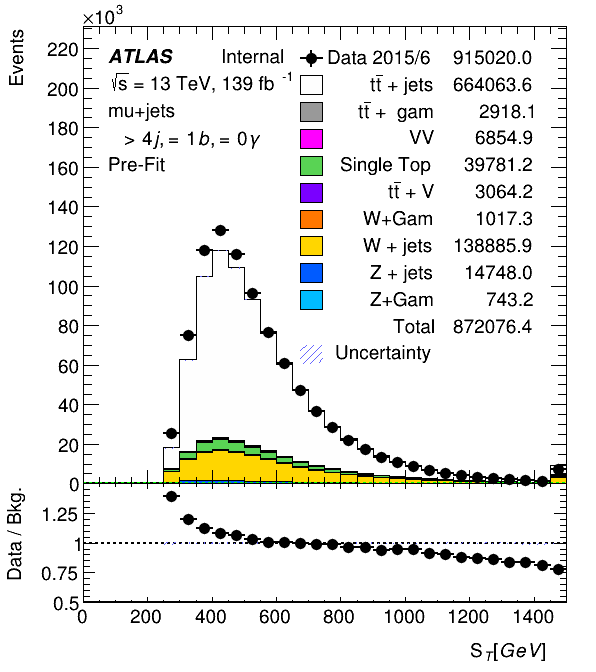
\includegraphics[width=.33\columnwidth]{../ThesisImages/RegionPlots/AfterScaling/ControlRegions/HardCodedNormFactor/FCNC_All_mujets/Plots/CR2_ST.png}}
\caption{$S_T$ distributions in the 3(a,d), 4(b,e), and 5+(c,f) jets control and validation regions. Electron channel is shown on the top and the muon channel on the bottom, before scale factors are determined.}
\label{fig:CRSTs}
\end{figure}

The efficiency of scale factors derived using control regions 1 ($n_{\text{jets}}$=3) and 2 ($n_{\text{jets}}\geq$5) are then tested in the validation region ($n_{\text{jets}}$=4).  The scale factors for the $t\bar{t}$ and W+jets MC are derived using:
\[ 
\begin{bmatrix}  
N(W)_{3j} & N(t\bar{t})_{3j} \\ N(W)_{5+j} & N(t\bar{t})_{5+j} \end{bmatrix} \begin{bmatrix} W_{SF} \\ t\bar{t}_{SF} \end{bmatrix} =
 \begin{bmatrix} N(\text{data-bkg})_{3j} \\N(\text{data-bkg})_{5j} \end{bmatrix}
\]
Figure \ref{fig:CRSTs} shows the $S_T$ distribution in both electron and muon channels before scale factors are calculated for all three kinematically separate regions.  The large mismodelling occurs at low $S_T$ values as expected as QCD processes will typically add low energy jets to the events.  The  Figures \ref{fig:VR3ejpostscale}(electron channel) and \ref{fig:VR3mujpostscale}(muon channel) show various event-level variable plots for the validation region after the scale factors have been applied.

The derived scale factors using these regions are shown in Table \ref{tab:CR12SFs}
\begin{table}[h]
\begin{center}
{\renewcommand{\arraystretch}{1.2}
\begin{tabular}{ccc}
\hline
Sample     &  e+jets SF   & $\mu$+jets SF  \\  \hline 
W+jets    &  1.22   &  1.25	\\
$t\bar{t}$  &  1.06    &  1.01	\\ \hline
\end{tabular}
\caption{Derived $t\bar{t}$ and W+jets scale factors for QCD multijet backgrounds.  }
\label{tab:CR12SFs}
}
\end{center}
\end{table}


\begin{figure}[h!]
\centering
\subfloat[]{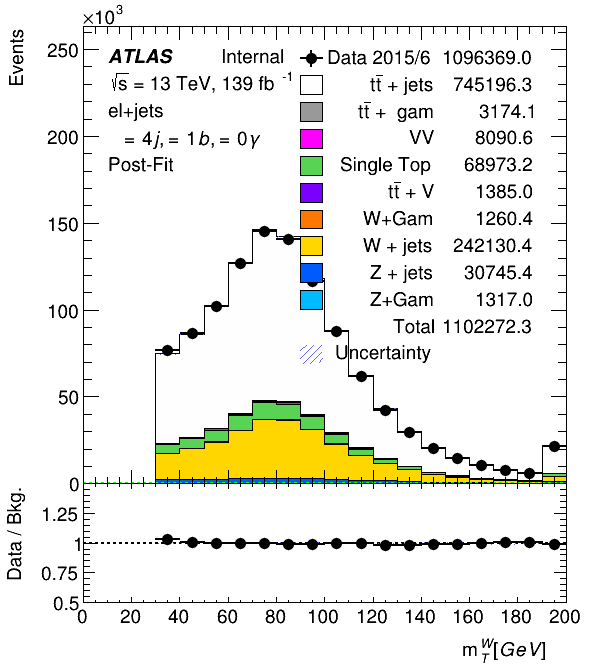
\includegraphics[width=.33\columnwidth]{../ThesisImages/RegionPlots/AfterScaling/ControlRegions/HardCodedNormFactor/FCNC_All_ejets/Plots/VR3_MWT_postFit.png}}\hfil
\subfloat[]{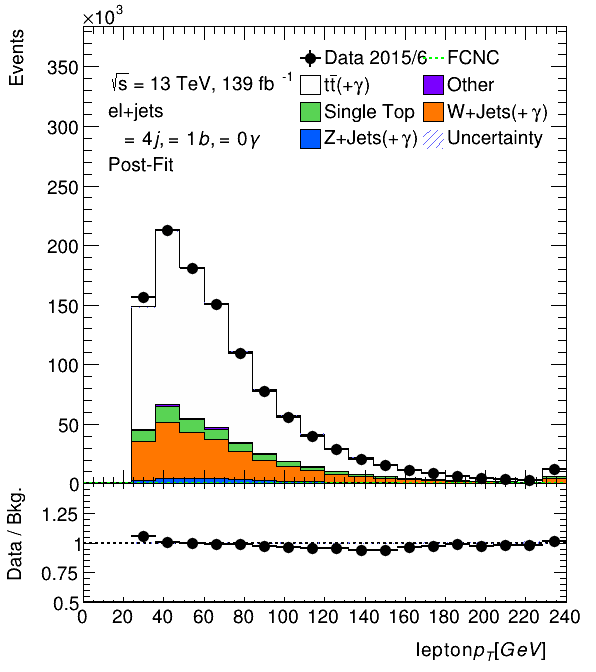
\includegraphics[width=.33\columnwidth]{../ThesisImages/RegionPlots/AfterScaling/ControlRegions/HardCodedNormFactor/FCNC_All_ejets/Plots/VR3_lep_pt_postFit.png}}\hfil  
\subfloat[]{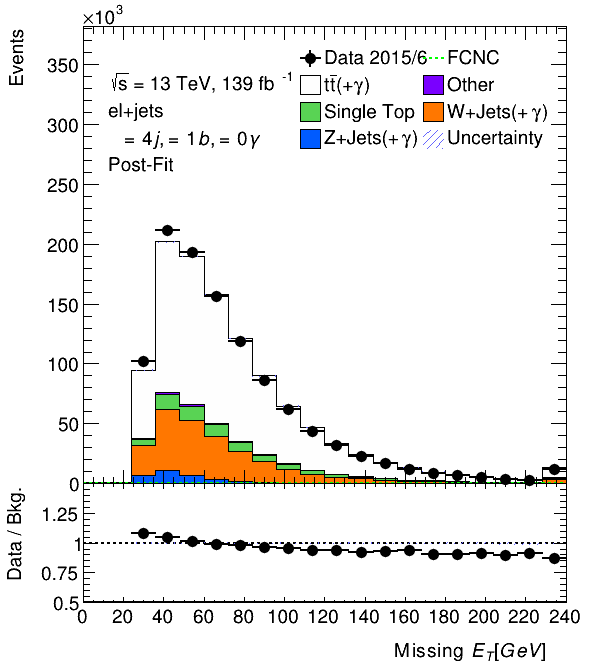
\includegraphics[width=.33\columnwidth]{../ThesisImages/RegionPlots/AfterScaling/ControlRegions/HardCodedNormFactor/FCNC_All_ejets/Plots/VR3_met_postFit.png}}
\vspace{-3.mm}
\subfloat[]{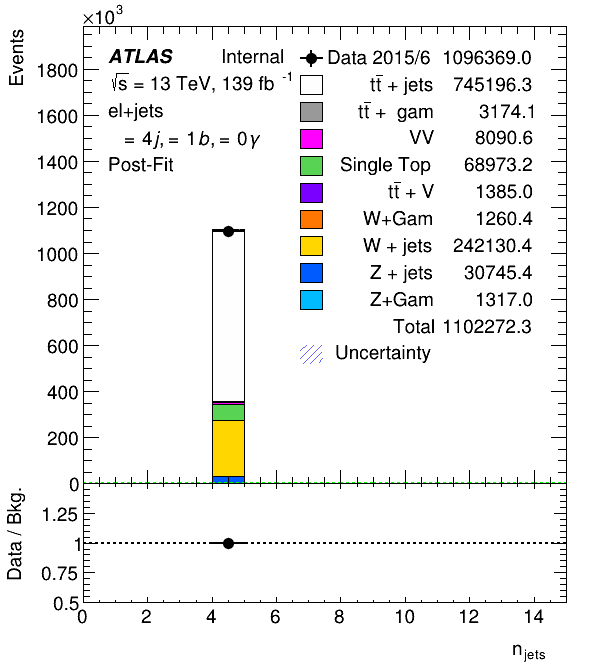
\includegraphics[width=.33\columnwidth]{../ThesisImages/RegionPlots/AfterScaling/ControlRegions/HardCodedNormFactor/FCNC_All_ejets/Plots/VR3_njet_postFit.png}}\hfil
\subfloat[]{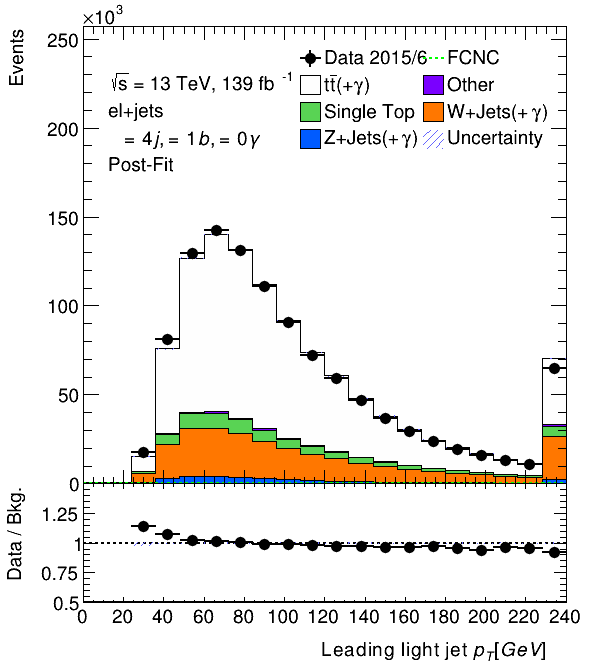
\includegraphics[width=.33\columnwidth]{../ThesisImages/RegionPlots/AfterScaling/ControlRegions/HardCodedNormFactor/FCNC_All_ejets/Plots/VR3_jet0_pt_postFit.png}}\hfil  
\subfloat[]{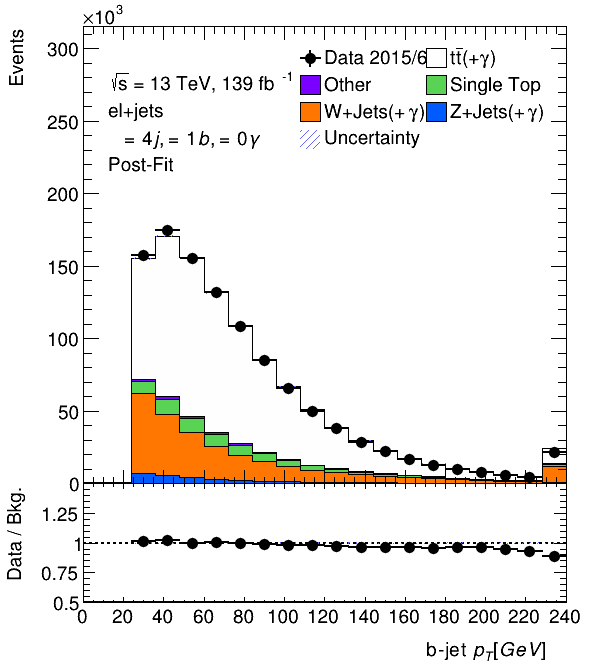
\includegraphics[width=.33\columnwidth]{../ThesisImages/RegionPlots/AfterScaling/ControlRegions/HardCodedNormFactor/FCNC_All_ejets/Plots/VR3_bjet0_pt_postFit.png}}
\caption{Event-level plots for the =4 jet validation region after scale factors have been applied in the electron channel.  FCNC signal branching ratio is scaled to 1\%.}
\label{fig:VR3ejpostscale}
\end{figure}

\begin{figure}[h!]
\centering
\subfloat[]{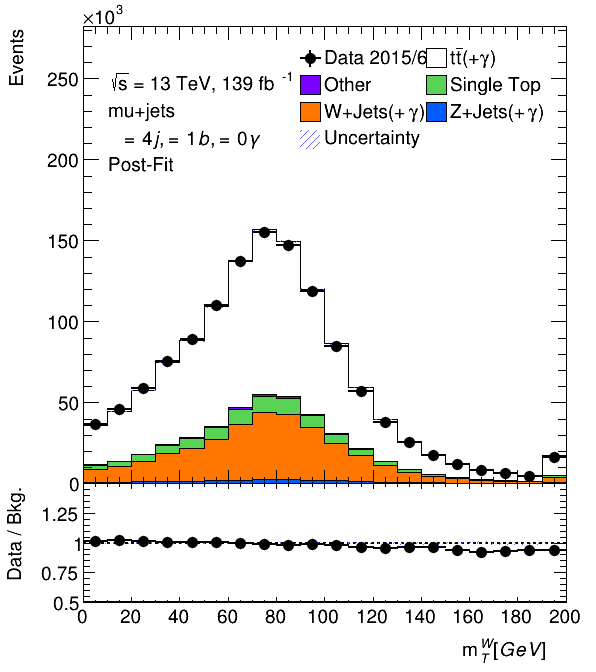
\includegraphics[width=.33\columnwidth]{../ThesisImages/RegionPlots/AfterScaling/ControlRegions/HardCodedNormFactor/FCNC_All_mujets/Plots/VR3_MWT_postFit.png}}\hfil
\subfloat[]{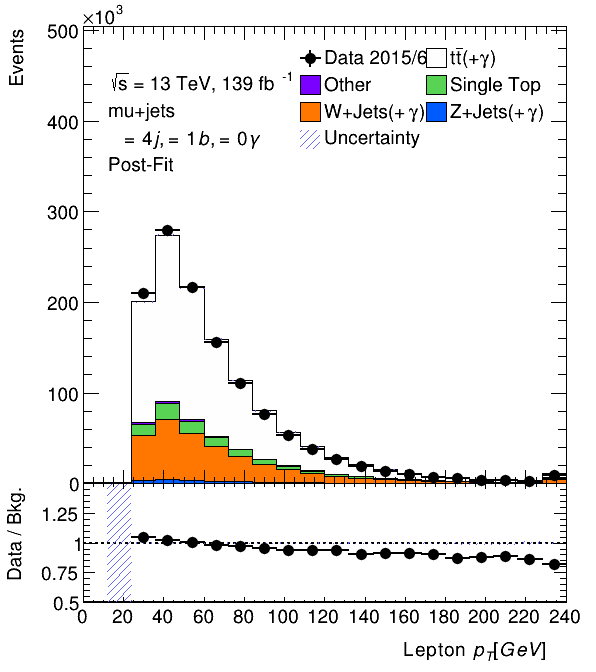
\includegraphics[width=.33\columnwidth]{../ThesisImages/RegionPlots/AfterScaling/ControlRegions/HardCodedNormFactor/FCNC_All_mujets/Plots/VR3_lep_pt_postFit.png}}\hfil 
\subfloat[]{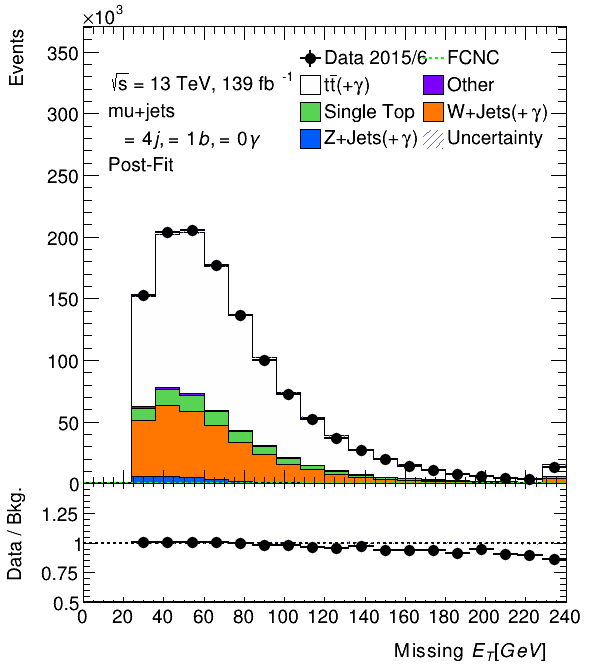
\includegraphics[width=.33\columnwidth]{../ThesisImages/RegionPlots/AfterScaling/ControlRegions/HardCodedNormFactor/FCNC_All_mujets/Plots/VR3_met_postFit.png}}
\vspace{-3.mm}
\subfloat[]{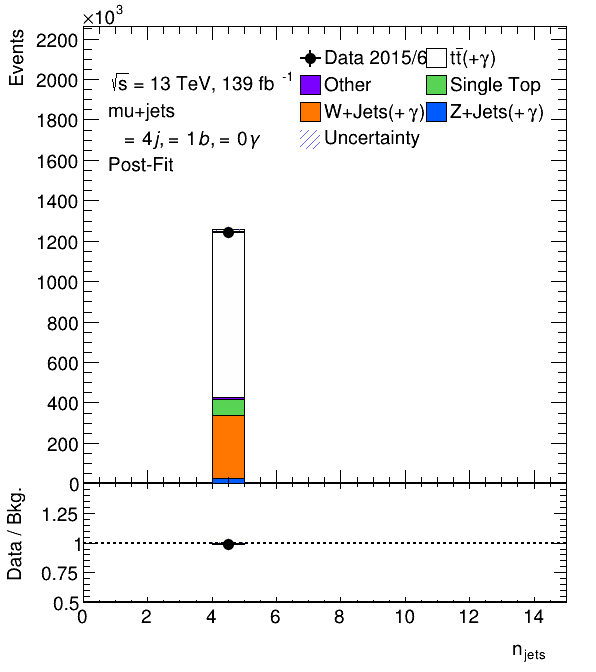
\includegraphics[width=.33\columnwidth]{../ThesisImages/RegionPlots/AfterScaling/ControlRegions/HardCodedNormFactor/FCNC_All_mujets/Plots/VR3_njet_postFit.png}}\hfil
\subfloat[]{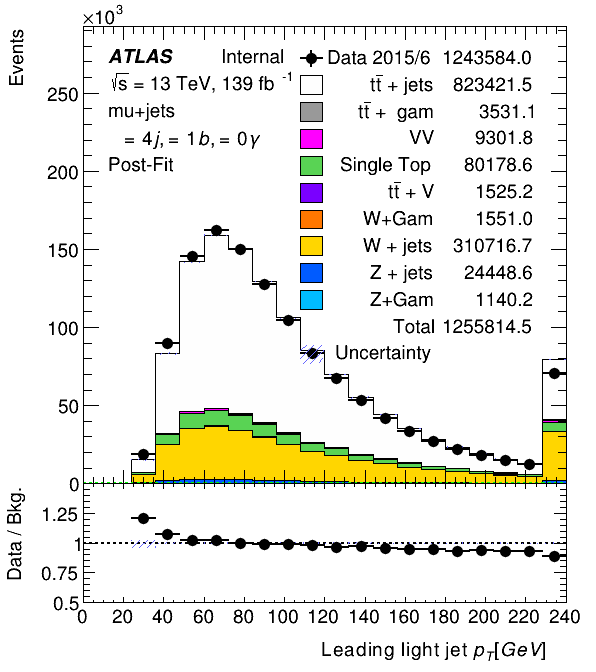
\includegraphics[width=.33\columnwidth]{../ThesisImages/RegionPlots/AfterScaling/ControlRegions/HardCodedNormFactor/FCNC_All_mujets/Plots/VR3_jet0_pt_postFit.png}}\hfil 
\subfloat[]{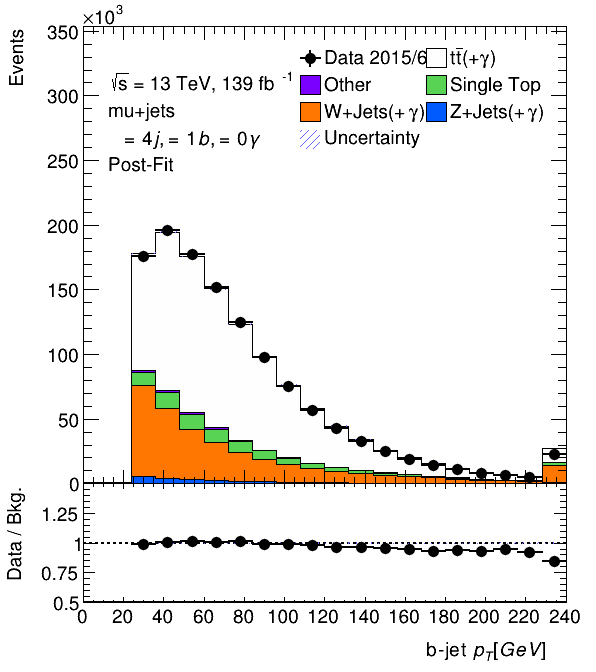
\includegraphics[width=.33\columnwidth]{../ThesisImages/RegionPlots/AfterScaling/ControlRegions/HardCodedNormFactor/FCNC_All_mujets/Plots/VR3_bjet0_pt_postFit.png}}
\caption{Event-level plots for the =4 jet validation region after scale factors have been applied in the muon channel.  FCNC signal branching ratio is scaled to 1\%.}
\label{fig:VR3mujpostscale}
\end{figure}


%%%%%%%%%%%%%%%%%%%%%%%%%%%%%%%%%%%%%%%%%%
%%%%%%%%%%%%%%%%%%%%%%%%%%%%%%%%%%%%%%%%%%
%%%%%%%%%%%%%%%%%%%%%%%%%%%%%%%%%%%%%%%%%%

\subsubsection{Background With Photons}
\label{sec:BKGPho}

Standard Model processes that are produced with an extra real photon are an irreducible background for this search as they can share the same final state as the signal events.  The largest contributors of these irreducible backgrounds are the major background samples discussed in the previous section with an associated photon ($t\bar{t}+\gamma$ and W+jets+$\gamma$).  Special Monte Carlo samples are produced for these samples (along with Z+jets+$\gamma$) that have higher statistics of these photon enriched events than the nominal samples.  However, as these samples (X+jets+$\gamma$) are subsets of the nominal sample(X+jets) duplicate events must be removed from the nominal sample.  This is done using the \textbf{MCTruthClassifier} tool which is detailed further in Section \ref{sec:Fakes}.  All events with a photon from the hard scattering are removed from the X+jets samples as they are contained within the X+jets+$\gamma$ samples.
\subsubsection{W+$\gamma$ Control Region}
A validation region for W+jets+$\gamma$ was created as it is one of the more dominat backgrounds other than $t\bar{t}$ and $t\bar{t}+\gamma$ events.  The normalization for the W+jets+$\gamma$ validation region enters as a free parameter into the final fit. The region selection for the W+jets+$\gamma$ is as follows:
\begin{itemize}
\item All of the Initial Event Selection as outlined in Section \ref{sec:InitSelec}
\item Exactly 1 lepton (electron or muon) $p_T >$ 25 GeV
\item At least 2 Jets  ($p_T >$ 25 GeV) 
\item $\slashed{E}_T >$ 30 GeV and $m_T^W >$ 30 GeV (for events with electrons)
\item $\slashed{E}_T >$ 20 GeV and $\slashed{E}_T + m_T^W >$ 60 GeV (for events with muons)
\item Exactly 0 b-tagged jet (MV2c10, 77\% Working point)
\item Exactly 1 photons, $p_T >$ 50 GeV
\item Photon isolation cuts: topo$E_T$cone40<4 GeV
\item Z mass cut $|m_{l\gamma}-m_Z|V>$ 5 GeV
\end{itemize}

Distributions of kinematic variables in the electron (muon) channels are shown in Figure \ref{fig:VR1ej} (\ref{fig:VR1muj}).
\begin{table}[h]
\begin{center}
{\renewcommand{\arraystretch}{1.2}
\begin{tabular}{c|c|c}
\hline
Channel:     &  e+jets   & $\mu$+jets  \\  \hline 
W+jets+$\gamma$ SF    &  PUT IN VALUE   & PUT IN VALUE	\\ \hline  %Change Put in post fit values
\end{tabular}
\caption{Fit result W+jets+$\gamma$ normalization scale factors including both statistical and systematic uncertainties.  }
\label{tab:VR1SFs} 
}
\end{center}
\end{table}
%Change : Add Discussion on agreement, allowing normalization into fit, postfit plots instead?

\begin{figure}[h!]
\centering
\subfloat[]{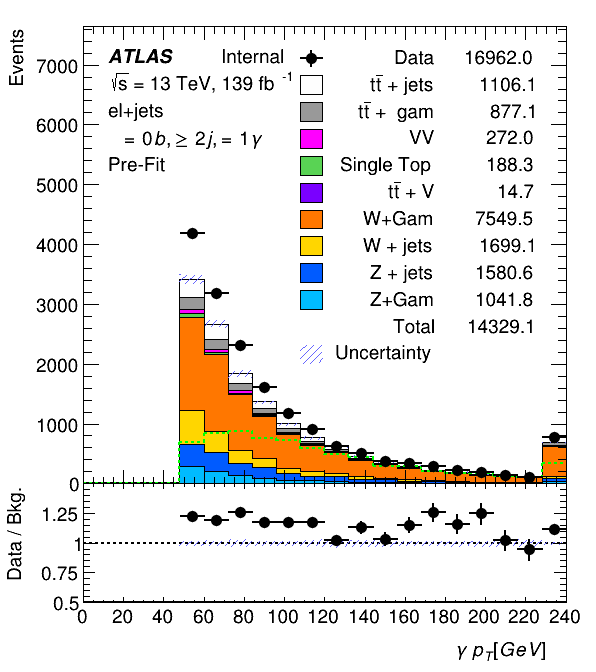
\includegraphics[width=.33\columnwidth]{../ThesisImages/RegionPlots/BeforeScaling/PhotonRegions/FCNC_All_ejets/Plots/VR1_ph_pt.png}}\hfil
\subfloat[]{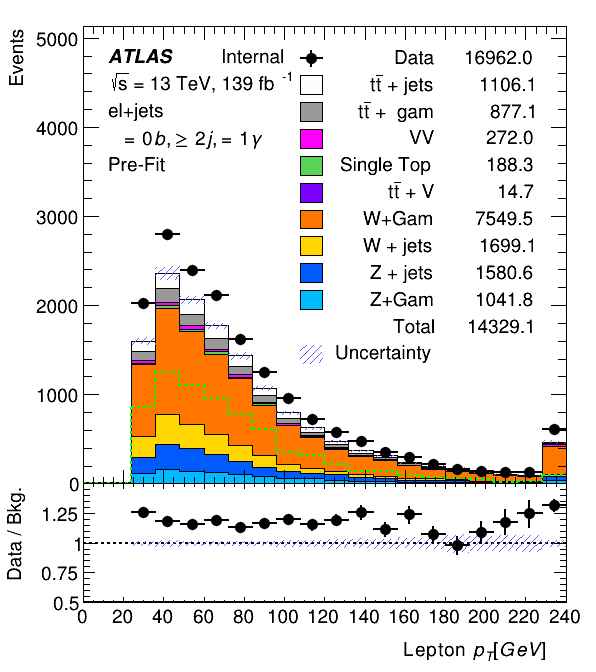
\includegraphics[width=.33\columnwidth]{../ThesisImages/RegionPlots/BeforeScaling/PhotonRegions/FCNC_All_ejets/Plots/VR1_lep_pt.png}}\hfil  %Change to AfterScaling
\subfloat[]{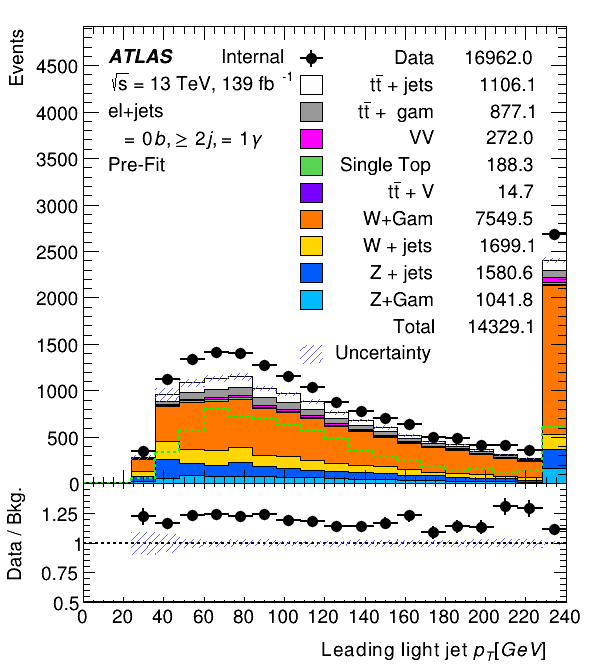
\includegraphics[width=.33\columnwidth]{../ThesisImages/RegionPlots/BeforeScaling/PhotonRegions/FCNC_All_ejets/Plots/VR1_jet0_pt.png}}
\vspace{-3.mm}
\subfloat[]{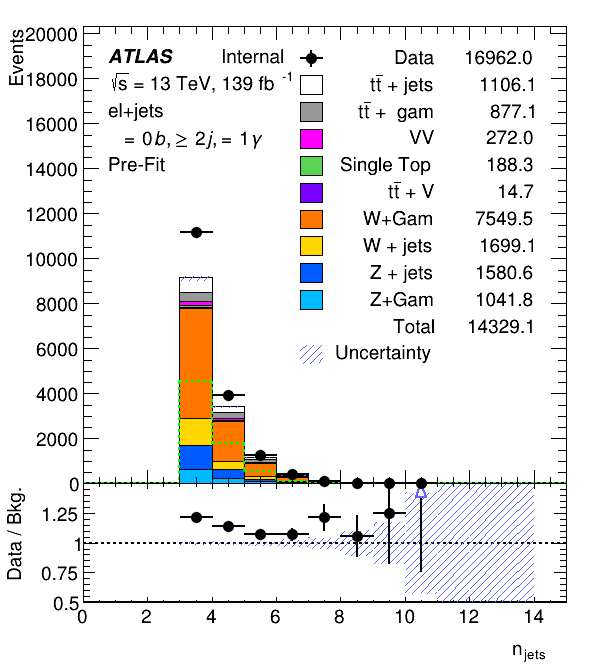
\includegraphics[width=.33\columnwidth]{../ThesisImages/RegionPlots/BeforeScaling/PhotonRegions/FCNC_All_ejets/Plots/VR1_njet.png}}\hfil
\subfloat[]{\includegraphics[width=.33\columnwidth]{../ThesisImages/RegionPlots/BeforeScaling/PhotonRegions/FCNC_All_ejets/Plots/VR1_MWT.png}}\hfil  %Change to AfterScaling
\subfloat[]{\includegraphics[width=.33\columnwidth]{../ThesisImages/RegionPlots/BeforeScaling/PhotonRegions/FCNC_All_ejets/Plots/VR1_ST.png}}
\caption{W+jets+$\gamma$ validation region plots for the electron channel.  The FCNC signal sample is scaled to 1\%.}
\label{fig:VR1ej}
\end{figure}

\begin{figure}[h!]
\centering
\subfloat[]{\includegraphics[width=.33\columnwidth]{../ThesisImages/RegionPlots/BeforeScaling/PhotonRegions/FCNC_All_mujets/Plots/VR1_ph_pt.png}}\hfil
\subfloat[]{\includegraphics[width=.33\columnwidth]{../ThesisImages/RegionPlots/BeforeScaling/PhotonRegions/FCNC_All_mujets/Plots/VR1_lep_pt.png}}\hfil  %Change to AfterScaling
\subfloat[]{\includegraphics[width=.33\columnwidth]{../ThesisImages/RegionPlots/BeforeScaling/PhotonRegions/FCNC_All_mujets/Plots/VR1_jet0_pt.png}}
\vspace{-3.mm}
\subfloat[]{\includegraphics[width=.33\columnwidth]{../ThesisImages/RegionPlots/BeforeScaling/PhotonRegions/FCNC_All_mujets/Plots/VR1_njet.png}}\hfil
\subfloat[]{\includegraphics[width=.33\columnwidth]{../ThesisImages/RegionPlots/BeforeScaling/PhotonRegions/FCNC_All_mujets/Plots/VR1_MWT.png}}\hfil  %Change to AfterScaling These are Prefit
\subfloat[]{\includegraphics[width=.33\columnwidth]{../ThesisImages/RegionPlots/BeforeScaling/PhotonRegions/FCNC_All_mujets/Plots/VR1_ST.png}}
\caption{W+jets+$\gamma$ validation region plots for the muon channel.  The FCNC signal sample is scaled to 1\%.}
\label{fig:VR1muj}
\end{figure}

\subsubsection{$t\bar{t}+\gamma$ Control Region}
Another validation region was created for the other largest photon enriched samples, $t\bar{t}+\gamma$. The normalization for the $t\bar{t}+\gamma$ validation region enters as a free parameter into the final fit and the region selection is as follows:
\begin{itemize}
\item All of the Initial Event Selection as outlined in Section \ref{sec:InitSelec}
\item Exactly 1 lepton (electron or muon) $p_T >$ 25 GeV
\item At least 4 Jets  ($p_T >$ 25 GeV) 
\item $\slashed{E}_T >$ 30 GeV and $m_T^W >$ 30 GeV (for events with electrons)
\item $\slashed{E}_T >$ 20 GeV and $\slashed{E}_T + m_T^W >$ 60 GeV (for events with muons)
\item At least 1 b-tagged jet (MV2c10, 77\% Working point)
\item Exactly 1 photons, $p_T >$ 50 GeV
\item Photon isolation cuts: topo$E_T$cone40<4 GeV
\item Reverse Neural Network Cut: NNOutput<0.93 electron channel, NNOutput<0.92 muon channel
\end{itemize}

Distributions of kinematic variables in the electron (muon) channels are shown in Figure \ref{fig:VR2ej} (\ref{fig:VR2muj}).
\begin{table}[h]
\begin{center}
{\renewcommand{\arraystretch}{1.2}
\begin{tabular}{c|c|c}
\hline
Channel:     &  e+jets   & $\mu$+jets  \\  \hline 
$t\bar{t}+\gamma$ SF    &  PUT IN VALUE   & PUT IN VALUE	\\ \hline %Change Put in post fit values
\end{tabular}
\caption{Fit result $t\bar{t}+\gamma$ normalization scale factors including both statistical and systematic uncertainties.  }
\label{tab:VR2SFs}
}
\end{center}
\end{table}
%Change : Add Discussion on agreement, allowing normalization into fit, change to postfit plots?

\begin{figure}[h!]
\centering
\subfloat[]{\includegraphics[width=.33\columnwidth]{../ThesisImages/RegionPlots/BeforeScaling/PhotonRegions/FCNC_All_ejets/Plots/VR2_ph_pt.png}}\hfil
\subfloat[]{\includegraphics[width=.33\columnwidth]{../ThesisImages/RegionPlots/BeforeScaling/PhotonRegions/FCNC_All_ejets/Plots/VR2_lep_pt.png}}\hfil  %Change to AfterScaling
\subfloat[]{\includegraphics[width=.33\columnwidth]{../ThesisImages/RegionPlots/BeforeScaling/PhotonRegions/FCNC_All_ejets/Plots/VR2_jet0_pt.png}}
\vspace{-3.mm}
\subfloat[]{\includegraphics[width=.33\columnwidth]{../ThesisImages/RegionPlots/BeforeScaling/PhotonRegions/FCNC_All_ejets/Plots/VR2_njet.png}}\hfil
\subfloat[]{\includegraphics[width=.33\columnwidth]{../ThesisImages/RegionPlots/BeforeScaling/PhotonRegions/FCNC_All_ejets/Plots/VR2_MWT.png}}\hfil  %Change to AfterScaling
\subfloat[]{\includegraphics[width=.33\columnwidth]{../ThesisImages/RegionPlots/BeforeScaling/PhotonRegions/FCNC_All_ejets/Plots/VR2_ST.png}}
\caption{$t\bar{t}$+jets+$\gamma$ validation region plots for the electron channel.  The FCNC signal sample is scaled to 1\%.}
\label{fig:VR2ej}
\end{figure}

\begin{figure}[h!]
\centering
\subfloat[]{\includegraphics[width=.33\columnwidth]{../ThesisImages/RegionPlots/BeforeScaling/PhotonRegions/FCNC_All_mujets/Plots/VR2_ph_pt.png}}\hfil
\subfloat[]{\includegraphics[width=.33\columnwidth]{../ThesisImages/RegionPlots/BeforeScaling/PhotonRegions/FCNC_All_mujets/Plots/VR2_lep_pt.png}}\hfil  %Change to AfterScaling
\subfloat[]{\includegraphics[width=.33\columnwidth]{../ThesisImages/RegionPlots/BeforeScaling/PhotonRegions/FCNC_All_mujets/Plots/VR2_jet0_pt.png}}
\vspace{-3.mm}
\subfloat[]{\includegraphics[width=.33\columnwidth]{../ThesisImages/RegionPlots/BeforeScaling/PhotonRegions/FCNC_All_mujets/Plots/VR2_njet.png}}\hfil
\subfloat[]{\includegraphics[width=.33\columnwidth]{../ThesisImages/RegionPlots/BeforeScaling/PhotonRegions/FCNC_All_mujets/Plots/VR2_MWT.png}}\hfil  %Change to AfterScaling
\subfloat[]{\includegraphics[width=.33\columnwidth]{../ThesisImages/RegionPlots/BeforeScaling/PhotonRegions/FCNC_All_mujets/Plots/VR2_ST.png}}
\caption{$t\bar{t}$+jets+$\gamma$ validation region plots for the muon channel.  The FCNC signal sample is scaled to 1\%.}
\label{fig:VR2muj}
\end{figure}